\documentclass{beamer}

\mode<presentation>
{
  \usetheme{default}
  \usecolortheme{default}
  \usefonttheme{default}
  \setbeamertemplate{navigation symbols}{}
  \setbeamertemplate{caption}[numbered]
  \setbeamertemplate{footline}[page number]
  \setbeamercolor{frametitle}{fg=white}
  \setbeamercolor{footline}{fg=black}
} 

\usepackage[english]{babel}
\usepackage[utf8x]{inputenc}
\usepackage{tikz}
\usepackage{listings}
\usepackage{courier}
\usepackage{array}
\usepackage{bold-extra}
\usepackage{minted}
\usepackage{dirtree}

\xdefinecolor{darkblue}{rgb}{0.1,0.1,0.7}
\xdefinecolor{darkgreen}{rgb}{0,0.5,0}
\xdefinecolor{darkgrey}{rgb}{0.35,0.35,0.35}
\xdefinecolor{darkorange}{rgb}{0.8,0.5,0}
\xdefinecolor{darkred}{rgb}{0.7,0,0}
\xdefinecolor{dianablue}{rgb}{0.18,0.24,0.31}
\definecolor{commentgreen}{rgb}{0,0.6,0}
\definecolor{stringmauve}{rgb}{0.58,0,0.82}

\lstset{ %
  backgroundcolor=\color{white},      % choose the background color
  basicstyle=\ttfamily\small,         % size of fonts used for the code
  breaklines=true,                    % automatic line breaking only at whitespace
  captionpos=b,                       % sets the caption-position to bottom
  commentstyle=\color{commentgreen},  % comment style
  escapeinside={\%*}{*)},             % if you want to add LaTeX within your code
  keywordstyle=\color{blue},          % keyword style
  stringstyle=\color{stringmauve},    % string literal style
  showstringspaces=false,
  showlines=true
}

\lstdefinelanguage{scala}{
  morekeywords={abstract,case,catch,class,def,%
    do,else,extends,false,final,finally,%
    for,if,implicit,import,match,mixin,%
    new,null,object,override,package,%
    private,protected,requires,return,sealed,%
    super,this,throw,trait,true,try,%
    type,val,var,while,with,yield},
  otherkeywords={=>,<-,<\%,<:,>:,\#,@},
  sensitive=true,
  morecomment=[l]{//},
  morecomment=[n]{/*}{*/},
  morestring=[b]",
  morestring=[b]',
  morestring=[b]"""
}

\title[2016-12-21-femtocode-odg]{Declarative query language for deeply nested data}
\author{Jim Pivarski}
\institute{Princeton University -- DIANA}
\date{December, 21, 2016}

\begin{document}

\logo{\pgfputat{\pgfxy(0.11, 8)}{\pgfbox[right,base]{\tikz{\filldraw[fill=dianablue, draw=none] (0 cm, 0 cm) rectangle (50 cm, 1 cm);}}}\pgfputat{\pgfxy(0.11, -0.6)}{\pgfbox[right,base]{\tikz{\filldraw[fill=dianablue, draw=none] (0 cm, 0 cm) rectangle (50 cm, 1 cm);}\tikz{\filldraw[fill=dianablue, draw=none] (0 cm, 0 cm) rectangle (4.9 cm, 1 cm);}}}}

\begin{frame}
  \titlepage
\end{frame}

\logo{\pgfputat{\pgfxy(0.11, 8)}{\pgfbox[right,base]{\tikz{\filldraw[fill=dianablue, draw=none] (0 cm, 0 cm) rectangle (50 cm, 1 cm);}}}}

% Uncomment these lines for an automatically generated outline.
%\begin{frame}{Outline}
%  \tableofcontents
%\end{frame}

%%%%%%%%%%%%%%%%%%%%%%%%%%%%%%%%%%%%%%%%%%%%%%%%%%%%%%%

%% \begin{frame}{I've been thinking about computational speed recently}
%% \vspace{0.5 cm}
%% \begin{itemize}\setlength{\itemsep}{0.25 cm}
%% \item Physicists have been thinking about single-processor efficiency for decades, and are beginning to think about scale-out.
%% \item Big Data community has been thinking about scale-out since it started, and is beginning to think about single-processor efficiency.
%% \vspace{0.1 cm}
%% \begin{itemize}\setlength{\itemsep}{0.1 cm}
%% \item Spark's Catalyst optimizer and Project Tungsten
%% \item Ibis, Impala, Kudu, Dremel/Drill\ldots
%% \end{itemize}
%% \item \textcolor{darkblue}{Speed is not a luxury:} the time between a query and its response limits a human data analyst's ability to develop instinct and see larger relationships.

%% \vspace{0.5 cm}
%% \textcolor{gray}{``Answers can change the question line\ldots\ every time.''}

%% \mbox{ } \hfill \textcolor{gray}{--- Adam Ant}
%% \end{itemize}
%% \end{frame}

%% \begin{frame}{Hurdle Theory}
%% \vspace{0.5 cm}
%% \textcolor{darkblue}{My favorite metaphor for computational speed:} fast software is not like a fast runner, who has some superior intrinsic ability. All programs run at the same rate, the clock rate. But some have more hurdles on the track than others.

%% \vspace{0.25 cm}
%% \begin{center}
%% 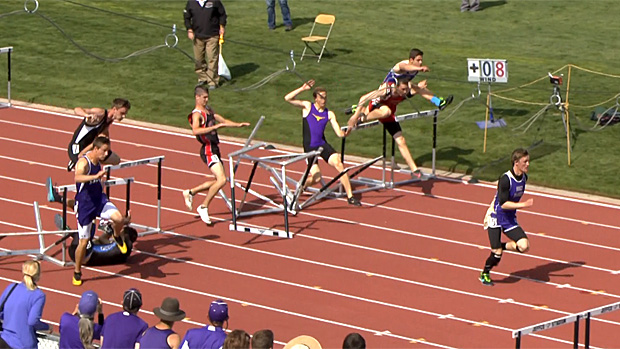
\includegraphics[width=0.7\linewidth]{hurdle9.jpg}
%% \end{center}
%% \end{frame}

%% \begin{frame}{But it's more than that\ldots}
%% \vspace{0.5 cm}
%% \begin{columns}
%% \column{0.4\linewidth}
%% 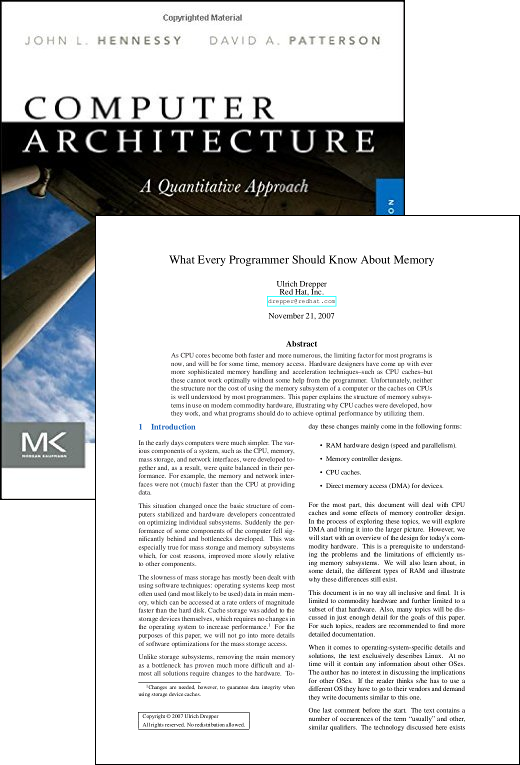
\includegraphics[width=\linewidth]{books.png}

%% \column{0.55\linewidth}
%% \textcolor{darkblue}{Gotcha: many of these hurdles are invisible!}

%% \vspace{0.5 cm}
%% Since the 90's, improvements in processor speed have outpaced improvements in memory bandwidth, so now memory is the bottleneck.

%% \vspace{0.5 cm}
%% Also, slow operations are pipelined to optimize throughput: many clock ticks from start to finish, but a full pipeline can push through one operation per clock tick.

%% \vspace{0.5 cm}
%% ``Bubbles'' in the pipeline \mbox{thwart this.\hspace{-1 cm}}
%% \end{columns}
%% \end{frame}

%% \begin{frame}[fragile]{What fast code looks like}
%% \vspace{0.5 cm}
%% \begin{center}
%% \begin{minipage}{0.7\linewidth}
%% \begin{minted}[frame=single]{c++}
%% for (int i = 0;  i < size;  i++)
%%   out[i] = in1[i] / in2[i];
%% \end{minted}
%% \end{minipage}
%% \end{center}

%% \begin{itemize}\setlength{\itemsep}{0.25 cm}
%% \item Simple loop structure that the compiler can unfold.
%% \item Forward stride that the CPU can detect and prefetch memory. (Arrays are contiguous in memory: bonus points for proper memory-alignment.)
%% \item Bubble-free pipeline (except at start and end; edge effects).
%% \item Would allow SIMD parallelism that could be vectorized \\ (1024 at once in a GPU, 4 or 8 for MMX, 256 for KNL\ldots).
%% \end{itemize}
%% \end{frame}

%% \begin{frame}{Field is ripe with low-hanging fruit}
%% \vspace{0.5 cm}
%% \textcolor{darkblue}{I've estimated that our weeks-long physics jobs, which touch hundreds of terabytes, could be reduced to minutes or seconds.}
%% \begin{itemize}
%% \item Only need to touch $\sim$80~GB of {\it columnar} data in typical 100 million event example.
%% \item {\it Single} processor can load 80~GB data arrays in 20~minutes \\ (so divide by $N$, number of processors).
%% \item Optimized C++ code can perform one simple operation in 12~seconds. (Divide by $N$.)
%% \item Low-end GPU can perform the same operation in 5~seconds. (Divide by $N$.)
%% \end{itemize}

%% \vspace{0.5 cm}
%% \small
%% \textcolor{gray}{Actually a change in behavior: ``weeks'' are spent making private skims to perform these operations quickly offline. But a shared server with sufficient caching would allow users to calculate one plot at a time, reducing the amount of data that needs to be read/copied.}
%% \end{frame}

%% \begin{frame}{Columns are essential}
%% \vspace{-1.5 cm}
%% \begin{itemize}\setlength{\itemsep}{0.25 cm}
%% \item Spark's Catalyst (SQL) optimizations and Project Tungsten (memory management) derive their benefit from columnar data and JIT-compilation.
%% \item \begin{minipage}[t]{0.5\linewidth}Even complex data structures can be represented as columns (``shredded'').\end{minipage}
%% \item \begin{minipage}[t]{0.5\linewidth}Mostly used to minimize disk access in file formats.\end{minipage}

%% \vspace{0.1 cm}
%% \begin{itemize}
%% \item Google Dremel
%% \item Apache Parquet
%% \item ROOT \textcolor{gray}{(physics, since 90's, unacknowledged in Google paper)}
%% \end{itemize}

%% \item Modern SQL engines are actually executing code on the raw columns, rather than reconstructing records.
%% \end{itemize}

%% \vspace{-5 cm}
%% \mbox{ } \hfill 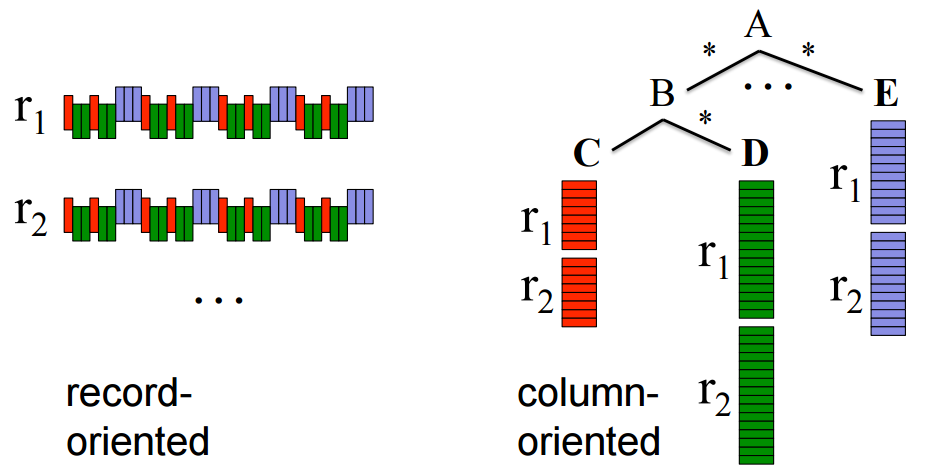
\includegraphics[width=0.4\linewidth]{columnar.png}
%% \end{frame}

%% \begin{frame}{But SQL is not expressive enough}
%% \vspace{0.5 cm}
%% \textcolor{darkblue}{Big irony:} modern DataFrames allow nested structure with clever shredding algorithms to work directly with raw columns, but SQL the language doesn't offer much for working with that structure.

%% \vspace{0.5 cm}
%% We discovered this while porting physics analyses to Spark: data are in DataFrames, but we can't do anything useful with them without dropping to RDDs.

%% \vspace{0.5 cm}
%% RDD access is ten times slower. Spark can't analyze Scala functions into work-plans.
%% \end{frame}

%% \begin{frame}[fragile]{Example: nested query in C++}
%% \vspace{0.25 cm}
%% \begin{center}
%% \begin{minipage}{0.95\linewidth}
%% \textcolor{darkblue}{``Momentum of the track with $|\eta|$ $<$ 2.4 that has the most hits.''}

%% \vspace{-0.5 cm}
%% \textcolor{darkblue}{\dirtree{%
%% .1 events.
%% .2 tracks.
%% .3 hits.
%% }}

%% \end{minipage}
%% \end{center}
%% \small
%% \begin{minted}{c++}
%% Track *best = NULL;
%% for (int i = 0;  i < tracks.size();  i++) {
%%   if (fabs(tracks[i]->eta) < 2.4)
%%     if (best == NULL ||
%%         tracks[i]->hits.size() > best->hits.size())
%%       best = tracks[i];
%% }
%% if (best != NULL)
%%   return best->pt;
%% else
%%   return 0.0;
%% \end{minted}

%% \vspace{0.1 cm}
%% \textcolor{gray}{(Something similar could be constructed for DNS queries or some other domain-specific structure.)}
%% \end{frame}

%% \begin{frame}[fragile]{Example: nested query in SQL}
%% \vspace{0.25 cm}
%% \begin{center}
%% \begin{minipage}{0.95\linewidth}
%% \textcolor{darkblue}{``Momentum of the track with $|\eta|$ $<$ 2.4 that has the most hits.''}
%% \end{minipage}
%% \end{center}
%% \small
%% \begin{minted}{sql}
%% WITH hit_stats AS (
%%   SELECT hit.track_id, COUNT(*) AS hit_count FROM hit
%%     GROUP BY hit.track_id),
%%  track_sorted AS (
%%     SELECT track.*, 
%%     ROW_NUMBER() OVER (
%%      PARTITION BY track.event_id
%%      ORDER BY hit_stats.hit_count DESC)
%%   track_ordinal FROM track INNER JOIN hit_stats
%%     ON hit_stats.track_id = track.id
%%     WHERE ABS(track.eta) < 2.4)
%%  SELECT * FROM event INNER JOIN track_sorted
%%    ON track_sorted.event_id = event.id
%% WHERE
%%   track_sorted.track_ordinal = 1
%% \end{minted}
%% \end{frame}

%% \begin{frame}[fragile]{Example: what it ought to look like}
%% \vspace{0.25 cm}
%% \begin{center}
%% \begin{minipage}{0.95\linewidth}
%% \textcolor{darkblue}{``Momentum of the track with $|\eta|$ $<$ 2.4 that has the most hits.''}
%% \end{minipage}
%% \end{center}
%% \small
%% \begin{onlyenv}<1>
%% \begin{minted}{bash}
%% tracks.filter(t => abs(t.eta) < 2.4)   # drop tracks
%%       .maxBy(t => t.hits.size)   # pick one (if any)
%%       .map(t => t.pt)            # transform it
%%       .impute(0.0)               # replace "None"
%%                                  # with a value
%% \end{minted}
%% \end{onlyenv}
%% \begin{onlyenv}<2>
%% \begin{minted}{bash}
%% tracks.filter(abs($1.eta) < 2.4)       # drop tracks
%%       .maxBy($1.hits.size)       # pick one (if any)
%%       .map($1.pt)                # transform it
%%       .impute(0.0)               # replace "None"
%%                                  # with a value
%% \end{minted}
%% \end{onlyenv}
%% \end{frame}

%% \begin{frame}{Summary}
%% \begin{description}
%% \item[SQL] is good at exploding data, but doesn't provide any support for rolling up transformed sublists. User has to create indexes and do ``joins'' (probably with a performance penalty).
%% \item[Scala/C++] can do anything, but performance is completely up to the user. The system can't examine a loop over events and rewrite it into vectorized operations on columns.
%% \item[Femtocode] is designed for this niche.
%% \end{description}
%% \end{frame}

%% \begin{frame}[fragile]{Femtocode is a unique language}
%% \vspace{0.25 cm}
%% \begin{itemize}
%% \item Provides an event-based, functional view of computation on identically typed, deeply structured data.
%% \item Rearranges the user's program to perform calculations on one columnar array at a time.
%% \end{itemize}

%% \begin{minted}{scala}
%% tracks.map(t => sqrt(t.px**2 + t.py**2)).max
%% \end{minted}

%% becomes

%% \vspace{-0.25 cm}
%% \begin{verbatim}
%% tmp1 := sqr(tracks.px)
%% tmp2 := sqr(tracks.py)
%% tmp3 := tmp1 + tmp2
%% tmp4 := sqrt(tmp3)
%% tmp5 := reduce.max(tmp4, tracks@size)
%% \end{verbatim}

%% where all of the above are arrays (and {\tt tmp5} has fewer entries than the rest).
%% \end{frame}

\begin{frame}{Some attributes of Femtocode, to make this possible}
\vspace{0.25 cm}
\begin{description}
\item[Declarative:] order written/order evaluated are often not the same.
\item[Functional:] map/filter/maxBy instead of explicit ``for'' loops.
\item[Vectorized:] operations on rows (e.g.\ events) transformed by compiler into operations on columns.

\item[No unbounded loops:] number of steps in each operation is finite and determined by the input data.

\item[No runtime errors:] any compileable query will return some result.

\item[Statically typed:] stronger type system than most languages is needed to eliminate runtime errors.

\item[Second-class functions:] functions may be partly passed as objects, but must be known at compile-time (same as PFA).

\item[No recursion/not Turing complete:] consequence of no unbounded loops. Femtocode belongs to a small class of ``total functional'' languages.
\end{description}
\end{frame}

\begin{frame}{Comparison to PFA}
\vspace{0.3 cm}
\begin{columns}[t]
\column{0.5\linewidth}
\textcolor{darkblue}{\underline{The same}}

\begin{itemize}
\item Limited language, focused on math, must be fed data from outside.

\item ``Two language solution:'' restricted PFA/Femtocode controlled by Scala/Python.

\item ``Second class functions'' with the same limitations.

\item Multiple execution engines adhering to a common standard.

\item Intermediate representation is JSON.
\end{itemize}

\column{0.5\linewidth}
\textcolor{darkblue}{\underline{Different}}

\begin{itemize}
\item Total functional and fully vectorizable.

\item Complete lack of runtime errors. \textcolor{gray}{\small (I started thinking about this while standardizing PFA: total functions are easier for guaranteeing conformance.)}

\item Femtocode has its own type system (not Avro).

\item Femtocode has a human-friendly syntax, based on Python.

\item API for users to add new {\it built-in} functions.
\end{itemize}

\end{columns}
\end{frame}

\begin{frame}{Execution engines}
\vspace{0.5 cm}
\textcolor{darkblue}{\underline{Planned}}

\begin{itemize}
\item C99 kernels for CPUs: accessible as a shared library in Python, Julia, Rust, etc. \textcolor{gray}{(Most languages have an FFI for shared libraries written in C, very few have hooks for C++.)}
\item Optimizations of some kernels for GPUs.
\item Execution engine for Numpy (requires Cython).
\item Execution engine for ROOT (requires ROOT).
\item Distributed server for physics data.
\end{itemize}

\vspace{0.25 cm}
\textcolor{darkblue}{\underline{Possible}}

\begin{itemize}
\item Java kernels on direct buffers. \textcolor{gray}{(No reason why a pure Java for loop on contiguous, off-heap data would be any \mbox{slower than C.)\hspace{-1 cm}}}
\item Execution engines for Spark DataFrames, Ibis, Impala, Kudu, Dremel, and the rest.
\end{itemize}
\end{frame}

\begin{frame}[fragile]{What data and execution kernels look like}
\vspace{0.5 cm}
\textcolor{gray}{(Active area of development: these are prototypes.)}
\small

\vspace{0.5 cm}
\begin{columns}
\column{0.4\linewidth}
\textcolor{darkblue}{\normalsize \underline{Schema}:}
\vspace{-0.1 cm}
\begin{minted}{python}
record(
  x=real,
  y=collection(
    record(
      a=real,
      b=collection(real)
      )))
\end{minted}

\column{0.5\linewidth}
\textcolor{darkblue}{\normalsize \underline{Input}:}
\vspace{-0.1 cm}
\begin{minted}{javascript}
[{x: 1.1, y: [
    {a: 2.2, b: [3.3, 4.4]},
    {a: 5.5, b: []}
    ]},
 {x: 6.6, y: [
    {a: 7.7, b: [8.8, 9.9]}
    ]}]
\end{minted}
\end{columns}

\vspace{0.5 cm}
\textcolor{darkblue}{\normalsize \underline{Resulting columns (``shredded'')}:}
\vspace{-0.1 cm}
\begin{minted}{python}
    "x":        [1.1, 6.6]            # flattened
    "y.a":      [2.2, 5.5, 7.7]
    "y.a@size": [2, 1]                # recursive walk
    "y.b":      [3.3, 4.4, 8.8, 9.9]
    "y.b@size": [2, 2, 0, 1, 2]       # recursive walk
\end{minted}
\end{frame}

\begin{frame}[fragile]{What data and execution kernels look like}
\vspace{0.5 cm}
\textcolor{gray}{(Active area of development: these are prototypes.)}
\small

\vspace{0.25 cm}
Operations can be performed on arrays at the same level of nesting without reference to their {\tt @size} arrays.

\vspace{0.25 cm}
\textcolor{darkblue}{\normalsize \underline{C99 for CPUs}:}
\vspace{-0.1 cm}
\begin{minted}{cuda}
void plus_ddd(int64_t len, double* in1array,
              double* in2array, double* outarray) {
  for (int64_t i = 0;  i < len;  i++)
    outarray[i] = in1array[i] + in2array[i];
}
\end{minted}

\vspace{0.25 cm}
\textcolor{darkblue}{\normalsize \underline{CUDA for GPUs}:}
\vspace{-0.1 cm}
\begin{minted}{cuda}
__global__
void plus_ddd(double* in1array, double* in2array,
              double* outarray) {
  int i = threadIdx.x;
  outarray[i] = in1array[i] + in2array[i];
}
\end{minted}
\end{frame}

\begin{frame}[fragile]{What data and execution kernels look like}
\scriptsize

\vspace{0.25 cm}
Consider the following Femtocode:
\begin{center}
\begin{minipage}{0.5\linewidth}
\begin{minted}[frame=single]{scala}
bias = one_per_event();
values.map(x => x + bias)
\end{minted}
\end{minipage}
\end{center}

The {\tt values} vector has a different length than {\tt bias} and must be interpreted with {\tt values@size}. Explode {\tt bias} to {\tt values}'s level.

\vspace{0.25 cm}
\textcolor{darkblue}{\small \underline{Explode function (prototype in Python)}:}
\begin{minted}{python}
def explode(modeldepth, modelsize, data, out):
    "Explode data to out with new size array modelsize."
    countdown = [None] * modeldepth
    cdi = 0; datai = 0; outi = 0
    for ms in modelsize:
        countdown[cdi] = ms
        if cdi == modeldepth - 1:
            while countdown[cdi] != 0:
                out[outi] = data[datai]; outi += 1
                countdown[cdi] -= 1
        if countdown[cdi] != 0:
            countdown[cdi] -= 1
        else:
            while cdi != -1 and countdown[cdi] == 0: cdi -= 1
        if cdi == -1: datai += 1
        cdi += 1
\end{minted}
\end{frame}

\end{document}




%% \begin{frame}{Two ways to more incisive data analysis}
%% \begin{columns}[t]
%% \column{0.5\linewidth}
%% \textcolor{darkblue}{\underline{Rapid, interactive queries}}
%% \vspace{0.2 cm}
%% Speed is not a luxury: the time between question and response limits a human's ability to understand and act on it.
%% \vspace{0.2 cm}
%% The reason you asked the question is still in mind.
%% \vspace{0.2 cm}
%% \begin{uncoverenv}<2->
%% \begin{itemize}
%% \item Ibis, Impala, Kudu, Drill\ldots
%% \item Usually SQL-like language
%% \item SparkSQL DataFrames
%% \end{itemize}
%% \end{uncoverenv}
%% \column{0.5\linewidth}
%% \textcolor{darkblue}{\underline{Deep manipulation}}
%% \vspace{0.2 cm}
%% Not all datasets are flat tables, especially ``data lakes'' shared for multiple purposes.
%% \vspace{0.2 cm}
%% Restructuring opens the door to finding new purposes for old data.
%% \vspace{0.2 cm}
%% \begin{uncoverenv}<2->
%% \begin{itemize}
%% \item Hadoop, PFA, custom code
%% \item ``Deployed analytic''
%% \item Spark RDDs and Datasets
%% \end{itemize}
%% \end{uncoverenv}
%% \end{columns}
%% \end{frame}
